The Bluetooth stack is composed of several layers \ref{fig:bt_stack}. For this project the important layers are the HCI, LMP, and the physical layer(Bluetooth Radio). The LMP have already been discussed in \ref{subsubsec:pairingprocess}. The HCI and the physical layer will be discussed below.

\begin{figure}[h]
  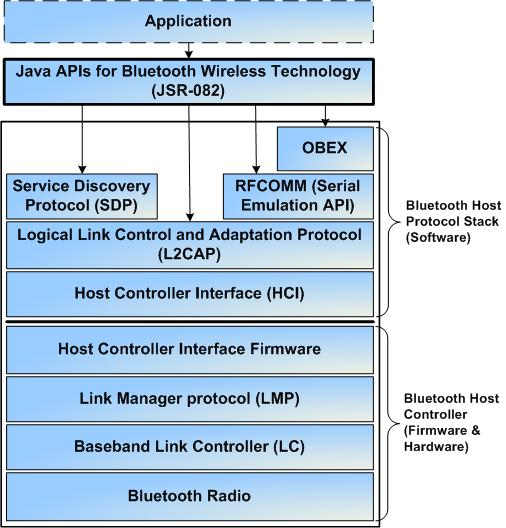
\includegraphics[scale=0.8]{images/bluetoothstack.jpg}
  \caption{The Bluetooth stack}
  \label{fig:bt_stack}
  \captionsetup{font={footnotesize,bf,it}}
  \caption*{\url{http://www.oracle.com/technetwork/testcontent/fig1-1-158000.jpg}}
\end{figure}
\newpage
\subsubsection{RG layer}
	% How we Gather data form the ubertooth
In order to eavesdrop the Bluetooth communication on the RF layer(Radio Frequency), the Ubertooth One has been used. This device is able to decode packet from a targeted Bluetooth communication. \pend
The LAP was known for the two devices. As explained in the literature review, the Ubertooth tool retrieve the important parameters (UAP, clocks) used to sniff a connection thanks to that address. Once the tool was able to sniff and follow the communication between the two devices it was possible for it to decode packets.
In order to have relevant information the authors conducted experiments in a certain way. Indeed several captures have been performed recording:
\begin{itemize}
	\item The pairing process between the two devices
	\item The de-authentication process between two devices
	\item The exchange of different data formats (videos, pictures, notification) 
\end{itemize}
The exchange of different data formats has been done with the apps that can be installed through the Smart Connect app. For video we used the app called "Camera". For images we used the app called "Slide show". \pend The example apps only do very basic things. The ones we used are: Hello Active Low Power, Hello Layouts and Hello Notification. These are all part of the SDK provided by Sony.
No significant changes have been made to these example apps. The only changes are the strings that are send and sending the messages in an infinite loop to automatically generate traffic.

\subsubsection{HCI layer}
	% How we Gather data form the hci
Due to the increasing use of Bluetooth; Android, since Android 4.4, has added a functionality for developers to look at Bluetooth packets that pass the HCI layer. This tool monitors the Bluetooth traffic outputs it in pcaps logs. These can be read with Wireshark for example. These logs can be found in the root of your data directory and is called btsnoop\_hci\.log.\pend
The HCI layer is just above the LMP layer where authentication and encryption/encapsulation takes place. This can be seen in figure \ref{fig:bt_stack}. The data and messages exchanged at this layer are in clear text and packets are not encapsulated. This makes them easily identifiable and easy to monitor. \pend
The experiments performed above at the Physical layer has been performed in the same way (and at the same time) at the HCI layer. Both tools need to be run at the same time to compare the data.